\documentclass[10pt,a4paper]{article}
\usepackage[utf8]{inputenc}
\usepackage{amsmath}
\usepackage{amsfonts}
\usepackage{amssymb}
\usepackage{graphicx}
\title{CROAC: Counting and Recognition using Omnidirectional Acoustic Capture}
\author{Marcel Gietzmann-Sanders}
\begin{document}
\maketitle
\section{The Pond}
It's an hour past sunset and the rain has just subsided. I approach the pond - a vernal pool that will dry up sometime this summer - trying as best I can to be a ghost. Unfortunately the crinkling of leaves reveals my corporeality and a hush descends upon the pond. It is as if the frogs recognize that their rehearsal time is over and have gone backstage in a mist of whispers as they let me get seated in anticipation of the grand event. Groping about in the darkness, as I have put out my head torch, I find the most comfortable seat in the house - a patch of dirt nestled among the roots of an old maple tree - and settle in. On the walk of mile or so in I've already heard the spring peepers chirping in all their eagerness and bullfrogs announcing their grandiose dominion with their earthly croaks, but I know that what all but a taste of what is to come. So I settle back  and wait for the concert to start.

It begins with solitary croaks as the bolder of the frogs begin to test the air, seeing whether their audience still stirs. But soon enough their comrades join in and the sound begins to mount. Layer by layer I hear different species enter the ensemble. Region by region the pond gets louder and louder as the frogs regain their composure. Before I know it the air is so thick with sound I feel as if I could breath it in. 

In full chorus it is impossible for me to discern the individual voices that make up this extraordinary orchestra. Instead all my two ears receive is a wall of frenetic sound. Yet the physicist in me recognizes this as a mere illusion and as I sit there bathed in chirps and croaks and wheezes I relish the richness of the data before me. I know that what my ears hear as a single curtain is in fact a richly woven fabric of pitches, amplitudes, and phases - a mathematical puzzle waiting to be untangled and solved. I realize that every spring night, and many a summer one too, these frogs broadcast into the ether a whole host of information on position, counts, energy, species, and perhaps even lineage. All waiting to be deciphered by a discerning soul. And so as I sat there at the base of that maple tree, bathed in the ciphered data of my amphibian friends, I wondered what it would take to break the code of frogs. The adventure into mathematics, computation, and herpetology that ensued has brought me untold joy, and I hope that in the subsequent paragraphs I can give you little taste of that adventure too. 

\section{The Richness of Sound}
We begin with Figure 1 - nothing more than a picture of a wave. If you've ever plucked a guitar string you'll know that sound is the result of vibrations. When some object like a string, or a speaker, or your very own vocal chords vibrates that vibration translates into waves in the air which we then hear as sound. All sound is composed of these waves, so a good place to start in trying to understand how to pick the various sounds apart is to understand how each sound wave is different from the next. To do that we'll look to the richest source of sound that our ears find already intelligible - music. 

\begin{figure}[!htb]
\center{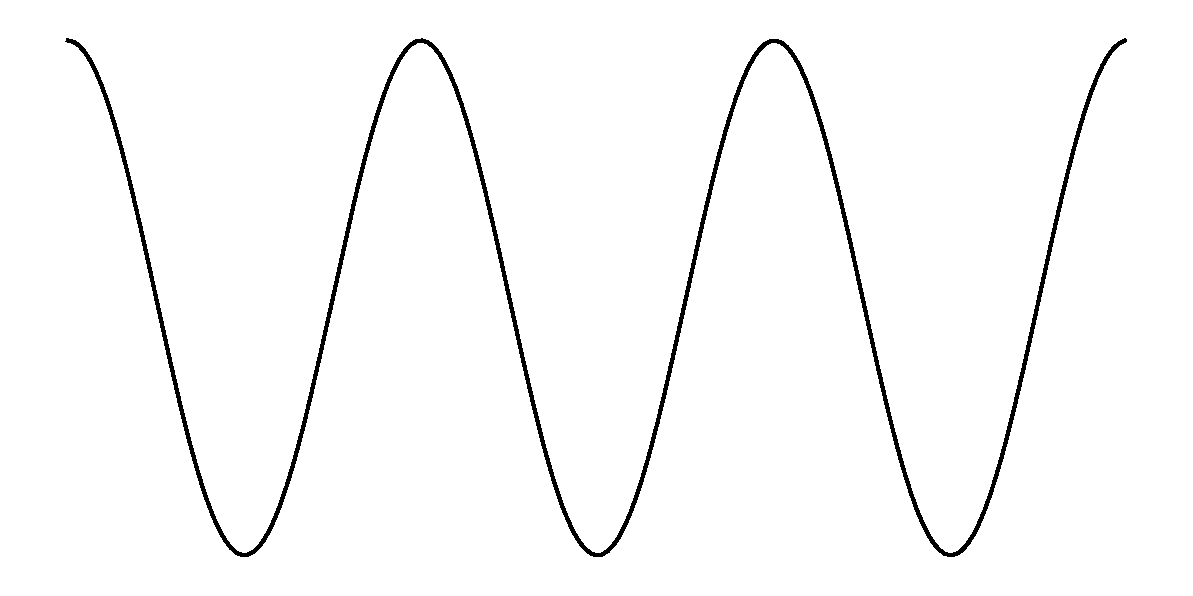
\includegraphics[width=\textwidth]
{figures/a_basic_wave.pdf}}
\caption{\label{fig:my-label} A Simple Wave}
\end{figure}

Music, as I just mentioned, is such a great place for us to begin understanding sound precisely because the human mind is already so used to picking out different sections, rhythms, and instruments - an activity quite similar to what we want to do with frog chorus. What can be much more difficult is picking out what your friends are trying to say when you're at a particularly loud concert. By the end of it you'll all have lost your voices given all the shouting you've done just to hear yourself. This, immediately, is our first discriminator - volume. As you raise your voice the volume of the sound that you are producing increases. Mathematically, volume is determined by the height of our wave - the farther the undulation has to go between each peak and valley the louder the sound is. This height is referred to as the \textbf{amplitude}. To visualize this, let's plot our simple wave but for the voices of two very different creatures - baleen whales and humans. 

Baleen whales are the largest animals to ever live and therefore, rather unsurprisingly, can be rather loud. To make the comparison really unfair and therefore even more astounding let's compare a rock concert to a blue whale. The typical sound level at a rock concert is around 110 decibels (dB) \cite{chris}. In comparison blue whales have been recorded at up to 180 dB \cite{zcormier}. This difference is actually far more ridiculous than it seems at first blush because of what a decibel actually is. When a decibel measurement increases by 10 that means the sound is around 3 \textit{times} louder. This means that our blue whale can be up to 21 times louder than a rock concert! To visualize just what a huge difference this is checkout Figure 2.

\begin{figure}[!htb]
\center{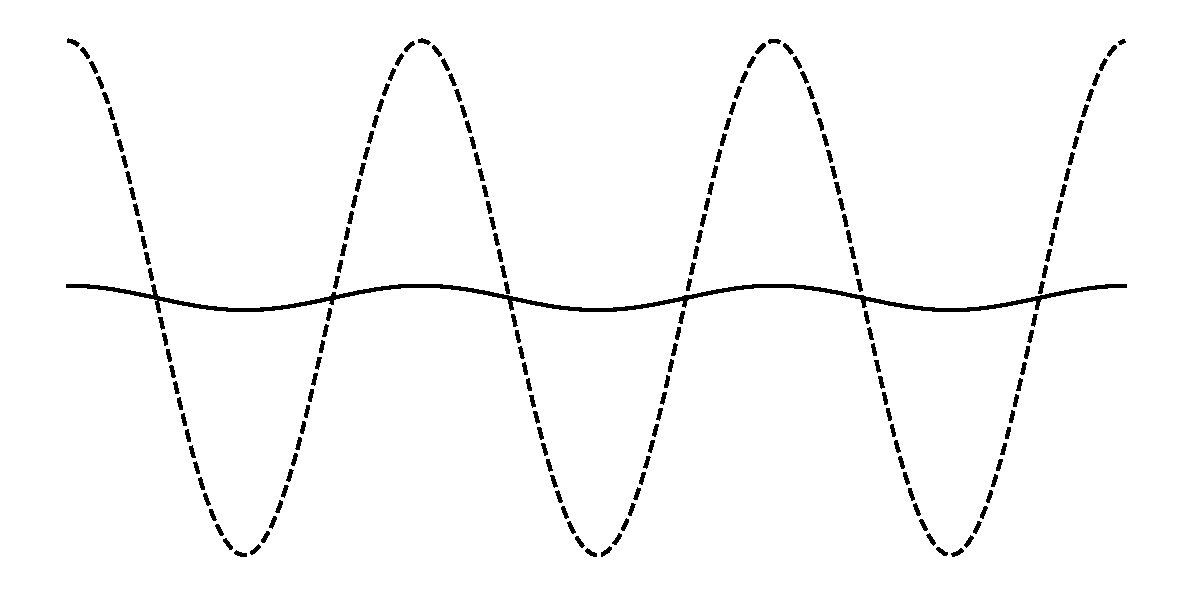
\includegraphics[width=\textwidth]
{figures/blue_whale_comparison.pdf}}
\caption{\label{fig:my-label} Blue Whale v. Rock Concert (dashed is the blue whale)}
\end{figure}

The dashed line represents the blue whale's amplitude whereas the solid line is the rock concert. There is such an amplitude difference that you can barely tell the solid line is a wave at all! It's barely a wiggle. 

Alright so that was amplitude which as we now know represents the volume of a sound. The next degree of freedom is exemplified by the fact that we can tell different instruments apart. For example, if you go and listen to an orchestra, even at the height of a piece when nearly all the instruments are playing together you can still tell the violins from the cellos. Why? Because the violins sound higher and the cellos lower. This is pitch. In contrast to amplitude which was how high our waves got, pitch is all about how wide they are. The distance from one peak to the next is called the \textbf{wavelength} and the larger that distance the lower the pitch of sound. Pitch however is rarely measured in wavelengths. Instead the standard measurement is Hertz (Hz) which is a unit of \textbf{frequency}. Frequency is simply the number of complete oscillations (peaks and troughs) per unit time. So, for example, when you hear that orchestras tune to A440 that 440 is actually 440 Hz. We can use the fact that we know the speed of sound $c$ to calculate the wavelength given the frequency. If $w$ is the wavelength and $k$ is the frequency then the conversion is simply:

\begin{equation}
w = c/k
\end{equation}

So if the speed of sound is 343 meters per second (m/s) then the wavelength of A440 is $343/440\approx0.78m$ or just over 2.5 feet. In comparison (visualized in Fig 3.) the highest note on a typical piano is at 7900 Hz \cite{wikipiano} which corresponds to a \textit{much} smaller wavelength ($343/7900=0.04m$).

\begin{figure}[!htb]
\center{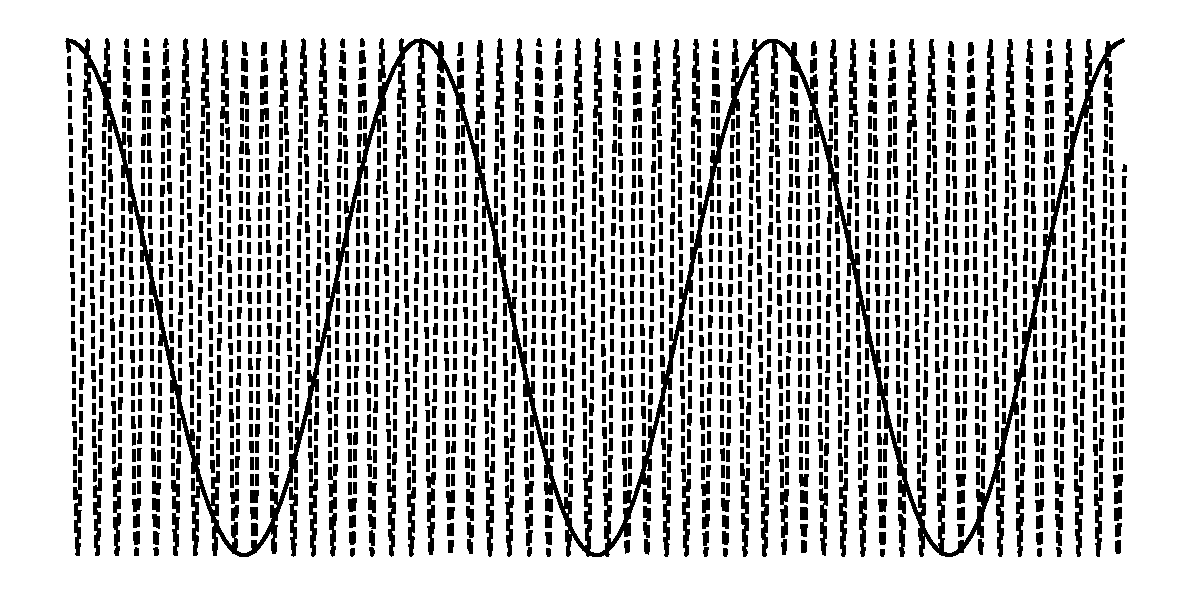
\includegraphics[width=\textwidth]
{figures/a440.pdf}}
\caption{\label{fig:my-label} A440 v. The Highest Note on a Piano (dashed is the higher note)}
\end{figure}

Now pitch can certainly explain how we can tell a violin apart from a cello, but what about instruments that have similar pitch? For example a piano and cello can play in the same range of pitches and yet you'd still be able to tell them apart. So what's going on here? Well so far we've been over simplifying things a lot. Remember how I said our picture of wave was the simplest picture possible? Well one of the ways in which it's super simple is that it's only got a single wavelength in it. In other words it has a single tone. Most sounds are not like this, most sounds have many wavelengths. This may sound pretty daft to you as I just described wavelength as the distance between peaks and now I'm saying there can be multiple distances between peaks, but the answer comes in the form of \textbf{superposition}. This is best illustrated by an example. 

All sounds "begin" with a fundamental frequency which is the lowest frequency tone in the sound. Then they'll have a series of higher tones built on top of that fundamental frequency. Each of these higher frequencies will usually have different amplitudes from both one another and the fundamental frequency. So let's begin with our simplest wave as the fundamental frequency (Fig 4.).

\begin{figure}[!htb]
\center{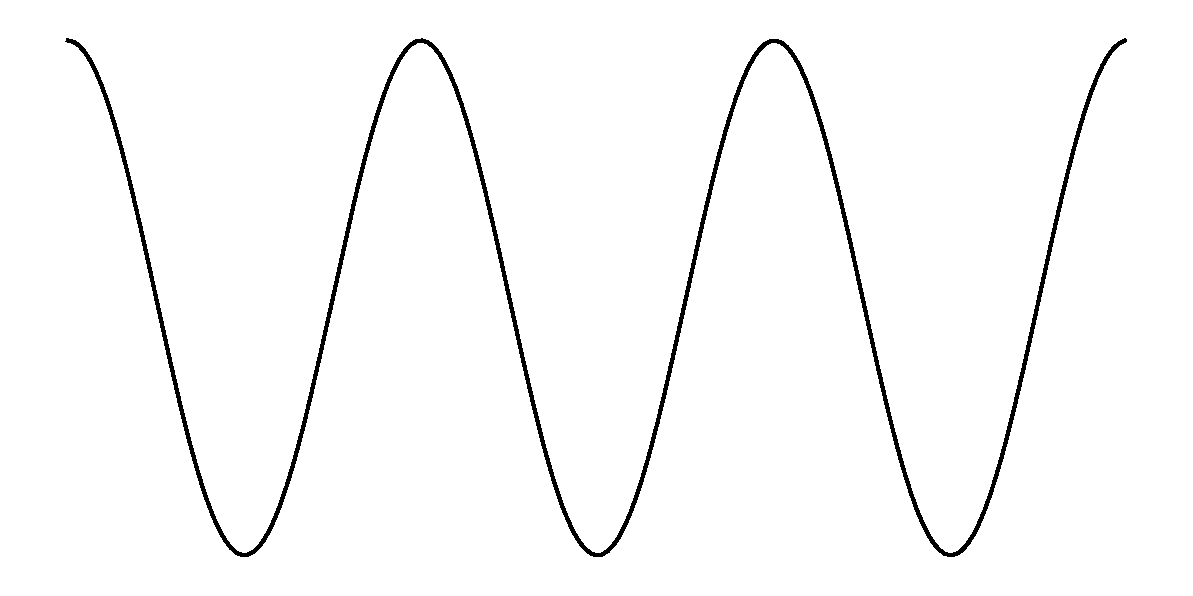
\includegraphics[width=\textwidth]
{figures/super1.pdf}}
\caption{\label{fig:my-label} Fundamental Frequency}
\end{figure}

Next we'll add in our first higher frequency, and we'll do so at half the wavelength and half the amplitude. Figure 5 shows both the two base waves (dashed) and the resulting superimposed wave (solid).

\begin{figure}[!htb]
\center{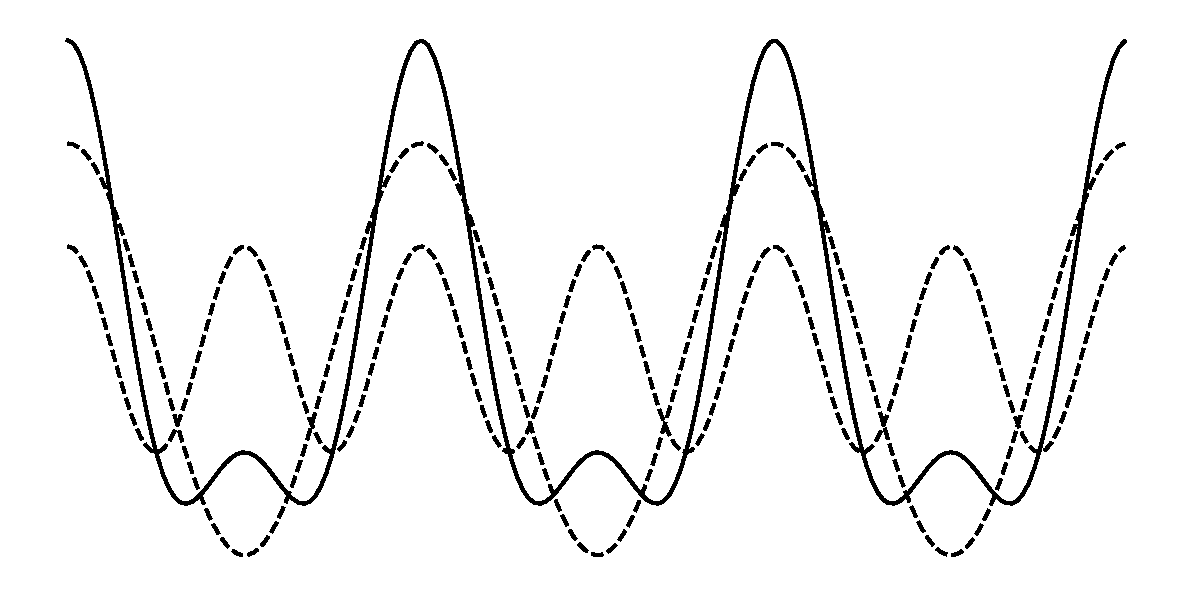
\includegraphics[width=\textwidth]
{figures/super2.pdf}}
\caption{\label{fig:my-label} Super Imposing Two Waves}
\end{figure}

Pretty wild right? Let's add one more frequency in, this time one quarter the wavelength of our fundamental frequency and equal in amplitude (Fig. 6). 

\begin{figure}[!htb]
\center{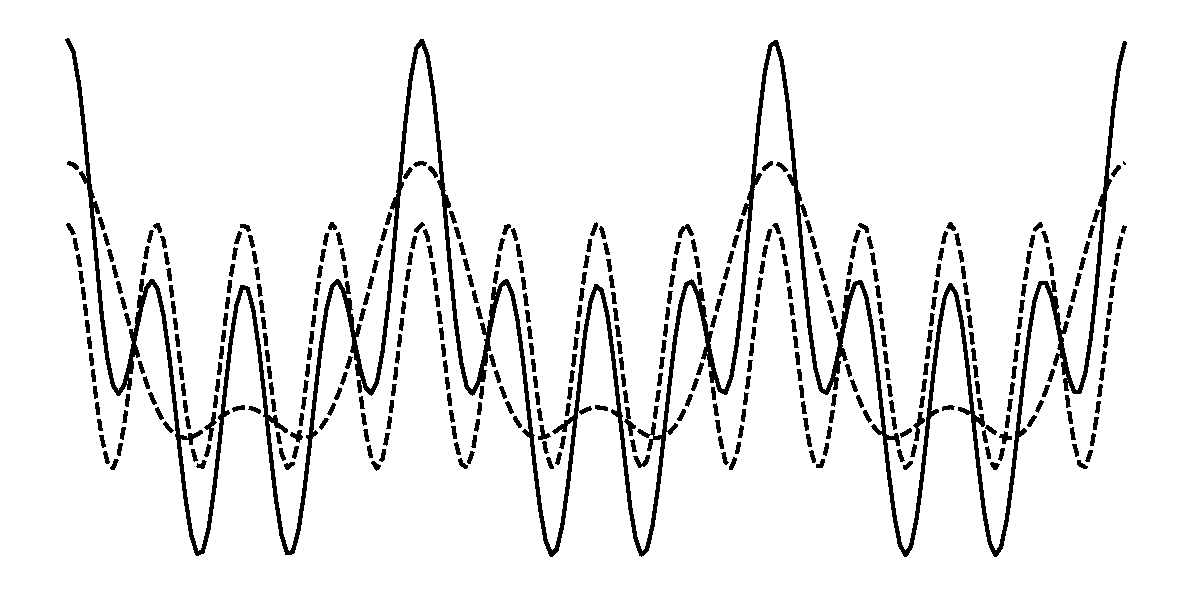
\includegraphics[width=\textwidth]
{figures/super3.pdf}}
\caption{\label{fig:my-label} Three Frequencies}
\end{figure}

Okay so this is cool and nerdy and all, but how does this relate back to distinguishing a piano from a cello and why do we care? Well when you play a note on any instrument the resulting sound is the superposition of whole load of different frequencies grounded on top of that fundamental frequency. Each instrument differs in exactly what that mix is and what the amplitudes of each frequency within the mix are. The combination particular to that instrument is therefore what gives the particular quality of sound that makes a piano sound different from a cello. For a trained ear, these differences can even allow you to identify one piano from another. For example if the higher pitches in the superposition have larger amplitude for one piano, then that piano will sound brighter. The particular mix of frequencies is thus another way to tell one sound from another.

Cool, so we've got amplitude, wavelength (and frequency), and superposition. Well there's one last component we can use in describing sound mathematically. I've saved this one for last because it's the most abstract and weird but one we're going to take advantage of a \textit{lot} - \textbf{phase}. 

So far we've been looking at all of these waves as being in one spot in our graph. But there's no reason why we can't start shifting them from left to right (Fig 7.). This shifting is phase. 

\begin{figure}[!htb]
\center{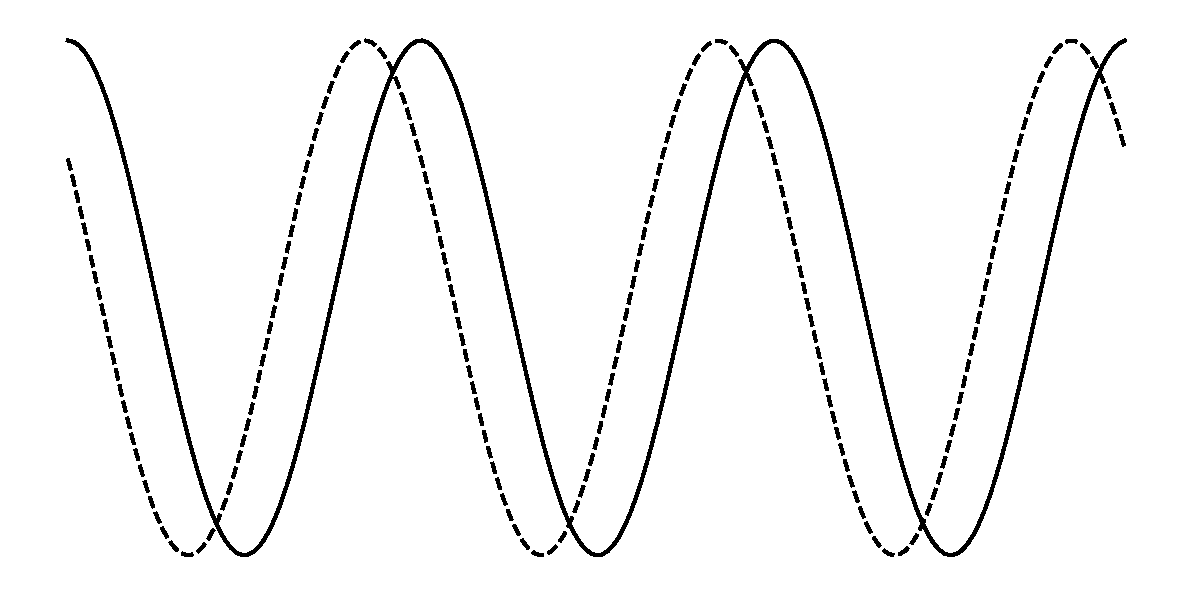
\includegraphics[width=\textwidth]
{figures/phase.pdf}}
\caption{\label{fig:my-label} Two Waves with Different Phases}
\end{figure}

What gets really weird and where we start to see the power of phase is when we superimpose two waves with the same wavelength and start varying the phase of just one. 

First Figure 8. shows the super position of the two waves from Fig 7. Note how because the waves are nearly in sync (peaks match with peaks and troughs match with troughs) they add together to create a wave with much higher amplitude. This is known as \textbf{constructive interference}.

\begin{figure}[!htb]
\center{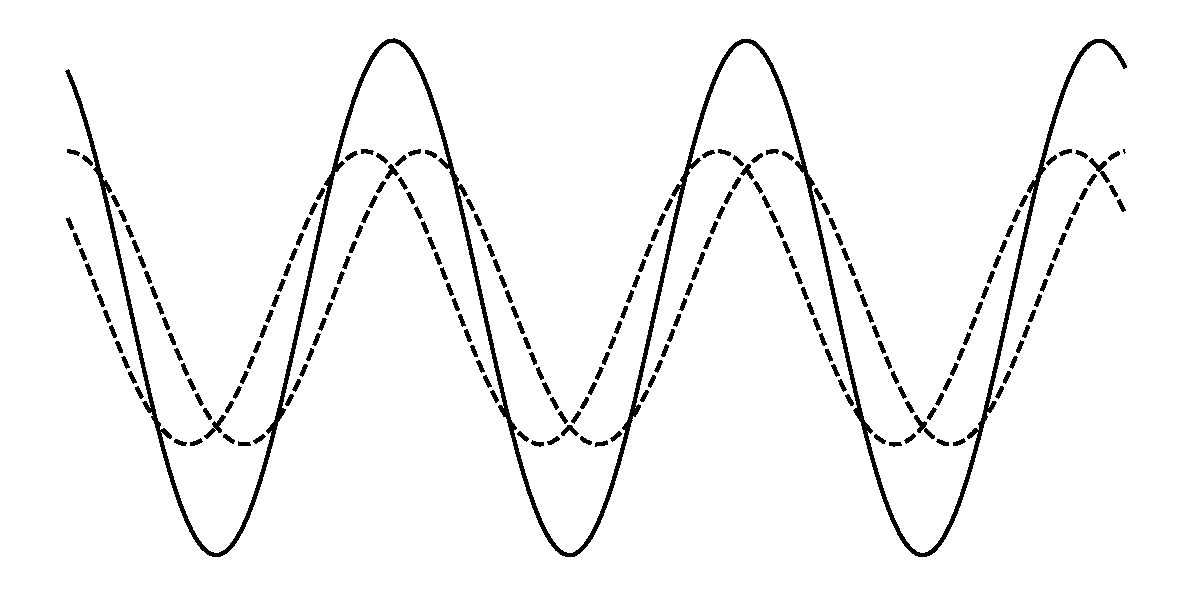
\includegraphics[width=\textwidth]
{figures/phasesuper1.pdf}}
\caption{\label{fig:my-label} Constructive Interference}
\end{figure}

On the other hand Figure 9 shows the superposition of two waves that are nearly out of sync (peaks at troughs and troughs at peaks). Note how in this case the resulting wave is much smaller than either of the constituents - this is \textbf{destructive interference}.

\begin{figure}[!htb]
\center{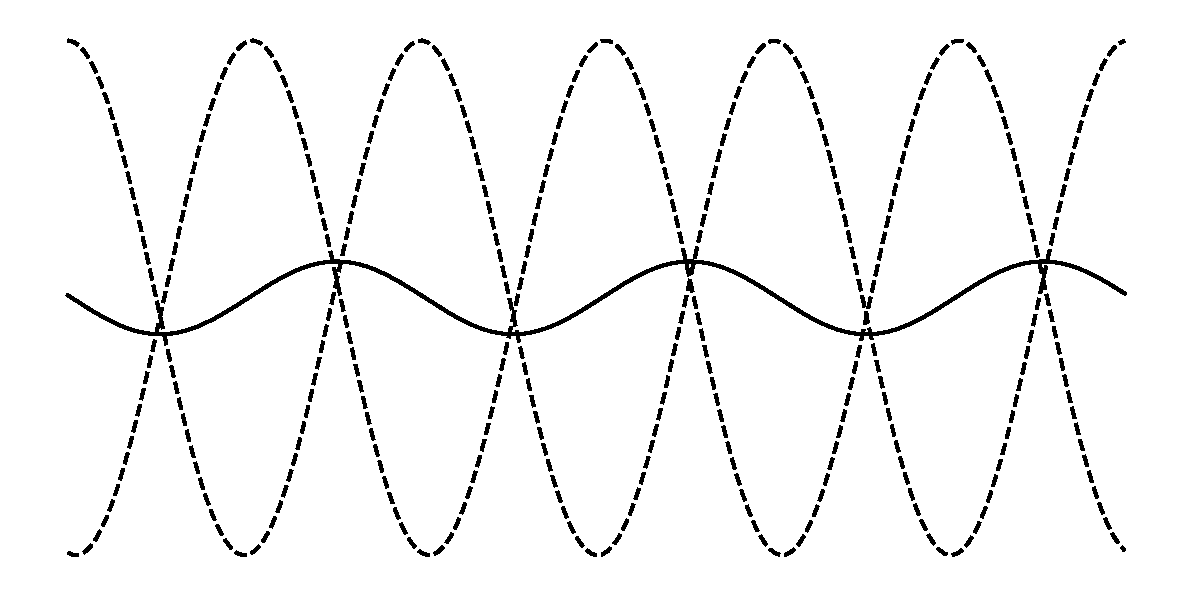
\includegraphics[width=\textwidth]
{figures/phasesuper2.pdf}}
\caption{\label{fig:my-label} Destructive Interference}
\end{figure}


What's really weird is that if you get the two waves to be exactly out of sync, the resulting superposition \textit{vanishes}! What does this mean physically? It means that the sound itself disappears! Yep, that's right, if two sound sources have just the right phase difference you'll suddenly no longer hear them even though the underlying sounds are there. Absolutely wild right? Even more wild is what happens when you consider the fact that you have two ears which are separated by the size of your brain. 

Suppose a sound is coming from directly to your right. That sound will obviously first hit your right ear. A very very short time later the same wave will hit your left ear, but at that point the undulation at your right ear will have changed. This difference in what your right and left ear are receiving is equivalent to the phase shift we were just talking about. Now suppose the sound is coming from directly in front of you. In this case the sound hits both ears at the same time because the distance to each ear is the same. This means there is no phase difference. Taken together we realize that as a sound source moves around your head the phase difference between your two ears changes. Ever wondered how it is you can tell the general direction a sound is coming from? This is how - your brain is picking up on small differences between each ear and sorting out what that means for the direction of the sound \cite{wikilocalization}. Pretty cool, right?! Well what we've just stumbled into is the simplest version of what's called a \textbf{phased array} which is what we'll dive into next. But before we can do that we need to summarize what we've learned and actually formalize it mathematically because phased arrays get pretty technical. So let's step back and do just that.

Alright, so we've got all our pieces:
\begin{itemize}
\item \textbf{Amplitude:} The height of a wave, representing volume.
\item \textbf{Wavelength (or Frequency):} The width of a wave, representing pitch.
\item \textbf{Superposition:} Many waves added together.
\item \textbf{Phase:} An abstract sense of the "position" of a wave that only becomes relevant during superposition.
\end{itemize}

How do we tie them all together mathematically? Well our simplest of waves is actually described by the following formula:
\begin{equation}
y=a e^{i\psi}e^{ikx}
\end{equation}
where $e=2.71828$ is a mathematical constant known as Euler's number, $i=\sqrt{-1}$ is the imaginary number, $a$ is our amplitude, $k=2\pi/w$ where $w$ is our wavelength, and $\psi$ (pronounced like \textit{sigh}) is our phase. That gets three of our four, but where is superposition? Well this is the equation for just one wave and superposition is many waves added together, so in order to get superposition we just add many waves together like so:
\begin{equation}
y = a_1 e^{i\psi_1}e^{ik_1x} + a_2 e^{i\psi_2}e^{ik_2x} + ... + a_N e^{i\psi_N}e^{ik_Nx}
\end{equation}
Now obviously writing out all these terms all of the time is going to get really clumsy and burdensome, so we're going to take advantage of a little bit of mathematical notation that you may or may not be familiar with - the sum $\Sigma$. For example if you were adding the numbers 1 through 100 you would normally write:
\begin{equation}
1 + 2 + 3 + ... + 100
\end{equation}
Which sucks to write out over and over again. So we'd represent this instead as:
\begin{equation}
\sum_{i=n}^{100}n
\end{equation}
which reads as - "add together all the $n$ where $n$ starts at 1 and goes all the way to 100". I appreciate that this is probably pretty abstract and a little mind bending if this is your first time seeing it, but as we dive further into our little adventure you'll see just how useful this one bit of notation is. And as the first example of the savings we get our:
\begin{equation}
y = a_1 e^{i\psi_1}e^{ik_1x} + a_2 e^{i\psi_2}e^{ik_2x} + ... + a_N e^{i\psi_N}e^{ik_Nx}
\end{equation}
can we be rewritten as:
\begin{equation}
y = \sum_{n=1}^{N}a_n e^{i\psi_n}e^{ik_nx}
\end{equation}
Which is far neater and as will become clear later, far easier to work with. 

\section{To Phase Array}
The one where we get into the math of phased arrays
\section{How Tall is A-flat?}
The one where we show how difficult sound is to work with
\section{The Fourth Dimension}
The one where we explain how we're going to get around sound's limitations
\section{A Frog in a Sound-stack}
The one where we explain the approach to the unsolved problem
\section{The Descent of Math}
The one where we work out the ML math
\section{Divergent Degenerates}
The one where we deal with some technical issues of our gradient
\section{We Did a Thing}
The one where we bring it all together
\section{What's Going On?}
The one where we reflect on what we achieved

\bibliographystyle{plain}
\bibliography{reference}

\end{document}